\begin{figure}
	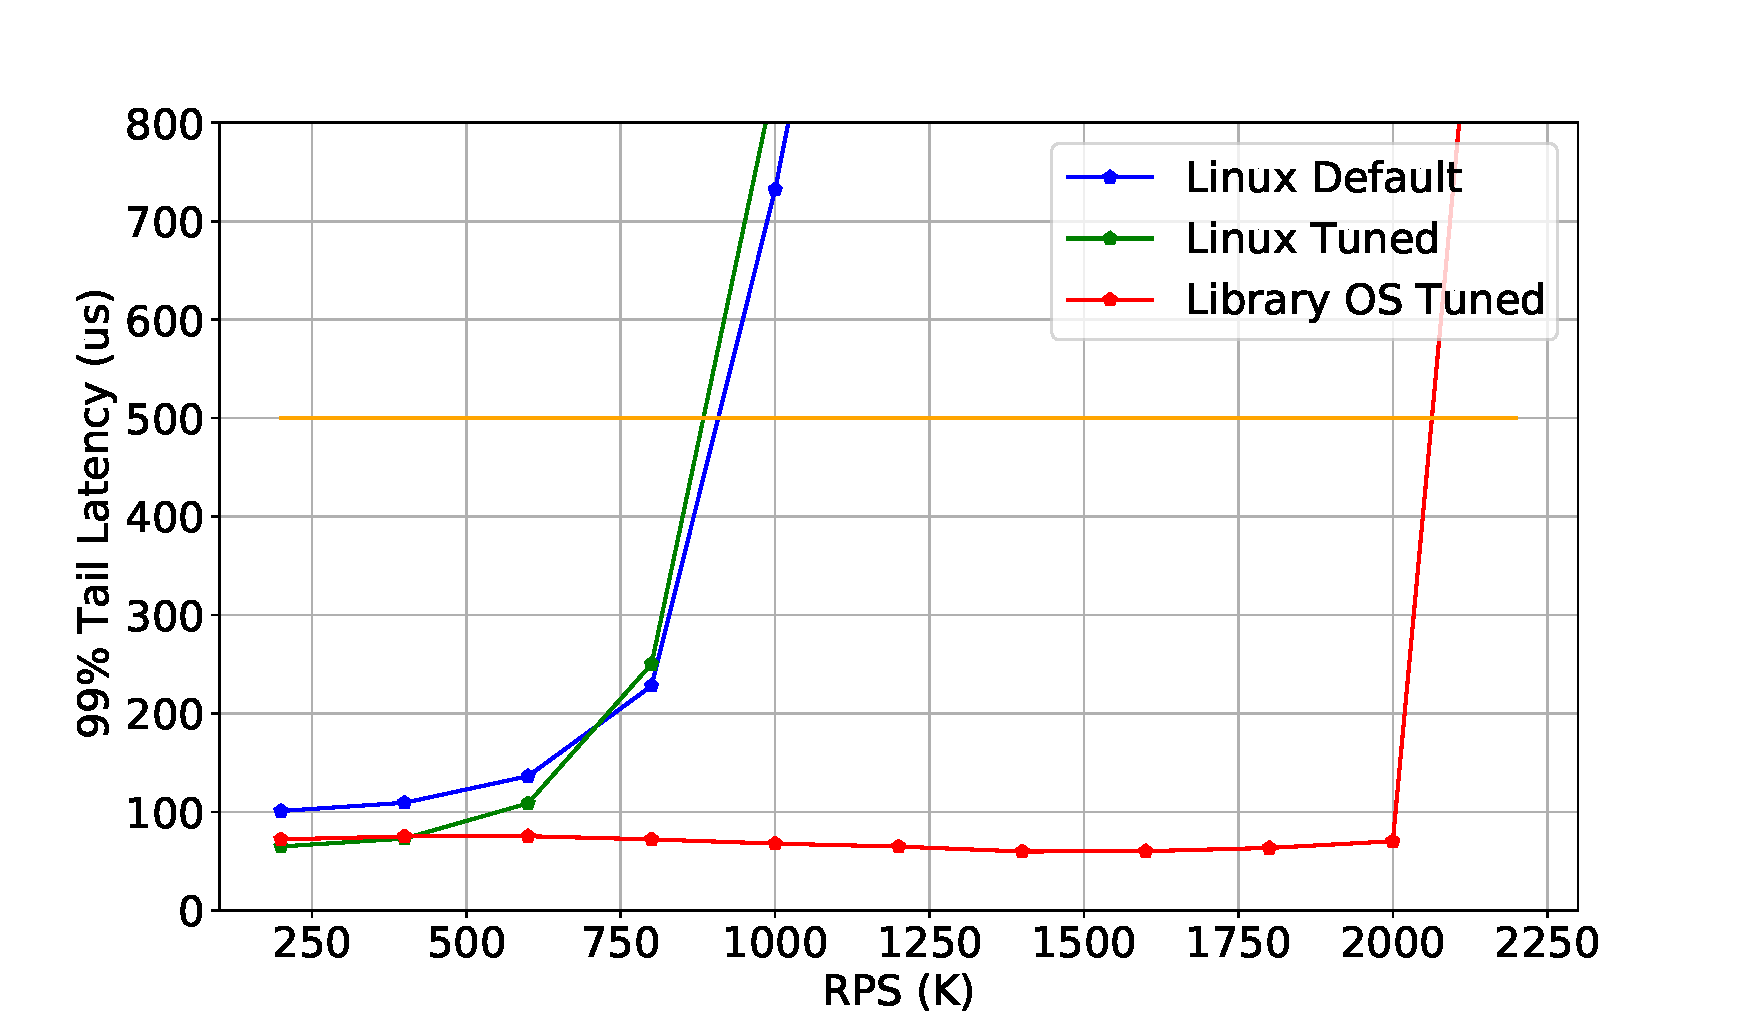
\includegraphics[width=\columnwidth]{asplos2021_figures/mcd_sla.pdf}
	\caption{Performance measure of memcached such that 99\% tail latency < 500 $\micro$s SLA. Compare default Linux with tuned for performance.}
	\label{fig:mcd_sla_tot}
\end{figure}



Figure~\ref{fig:mcd_sla_tot} compares the base performance between Linux default and the two systems when tuned for performance. Given that this is a complicated multicore workload with mixed requests rate and the need to satisfy a stringent SLA; tuning hardware parameters in Linux does not produce a noticeable increase in overall peak throughput (but does achieve lower tail latency at smaller QPS rates). This result is not surprising given the enormous efforts from past researchers to understand and optimize the network paths for workloads such as memcached~\cite{tailatscale, scalingmcdfacebook, workloadanalysisfacebook, ix, ebbrt, farm, 222583}. In contrast to Linux, the library OS uses a re-implemented version of memcached written to its interfaces and supports the standard memcached binary protocol. To alleviate lock contention, a RCU hashtable is used to store key-value pairs. While the library OS's implementation does lack some additional features such as authentication and other commands; it is functional enough to support the mutilate benchmark. The systems optimizations of the library OS coupled with a baremetal network device driver attributed in some part to 2X performance improvement over Linux.



%In contrast to the NAPI polling policy, EbbRT is not limited by a polling budget per receive interrupt, it will process as many receive descriptors as the hardware allows in a synchronous manner, moreover as interrupts are disabled during this entire process, EbbRT potentially could process more packets than Linux which must balance workload with processing budgets.
%Given the base performance of each system, f
%Figure~\ref{fig:mcd600K} illustrates the base energy costs when tuning Linux and library OS to minimize EDP. Similar to nodejs, we also scale the log data to show a fixed workload of 5 million requests for each system and the results we present below is for the 600K QPS rate. We noticed there was a discrepancy in the raw data logs only for Linux tuned in reported EDP values, therefore in figure~\ref{fig:mcd600K} we show the EDP for each run of all systems. It is something we are currently investigating.  However, the results we present regardless show significant differences in the system beyond the displayed variance.  

%While Memcached and the mutilate workload are more represented of a real world cloud service component and load.  It raises interesting challenges from an EDP analysis perspective.  Given that the benchmark generates the requests from a distribution over the request times (gets and sets of particular keys and data) there is no real fixed work rather it is a sample of work.  To this end we plot EDP curves from multiple runs given the observed variance.  While there is variance the optimized EDP shows distinct separation between the systems greater than the variance.  

% fixed tuning what kind of benefit over base Linux,
% what influence does having shorter code paths on tuning, 
% what does getting to sleep/idleness difference, 
% are you exploiting to sleep, synergistic with instruction efficiency,

%% \begin{figure}
%% 	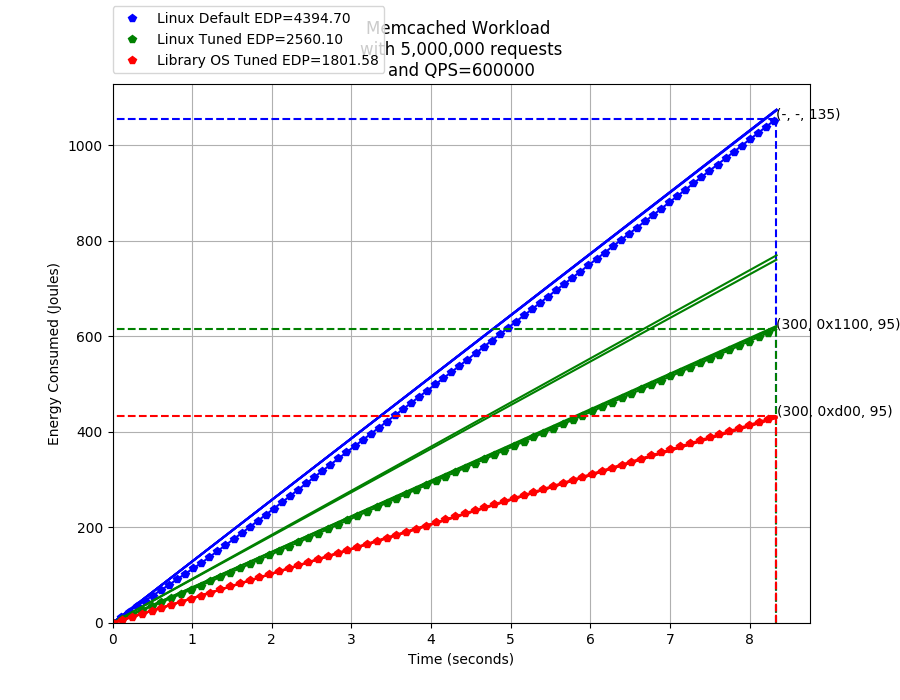
\includegraphics[width=\columnwidth]{asplos2021_figures/mcd_edp_QPS600000.png}
%% 	\caption{Minimum EDP plots when tuned for lowest energy use.}
%% 	\label{fig:mcd600K}
%% \end{figure}

%% \begin{figure}
%% 	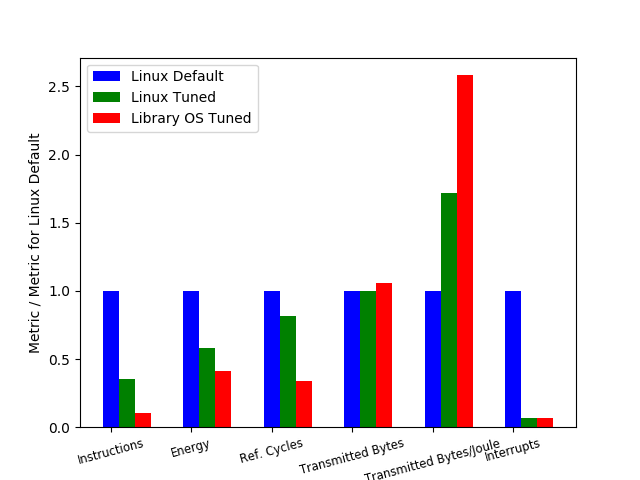
\includegraphics[width=\columnwidth]{asplos2021_figures/mcd_combined_barplot_QPS600000.png}
%% 	\caption{Summed up measures from logs and normalized against Linux default.}
%% 	\label{fig:mcdbar600K}
%% \end{figure}

As stated in the introduction there are dramatic energy saving when comparing the default Linux behavior to statically setting the hardware parameters as is evident in Figure~\ref{fig:mcd600K}.  Perhaps what is most surprising the trade-offs and causality observed in the simpler benchmarks result in a significant win under a far more complex load.  By-passing Linux default behaviour yields similar wins with respect to reducing the utilization between interrupts as indicated in Figure~\ref{fig:mcdnonidle600K}. Specifically, we find the improvement in interrupt processing leads respectively to decreases in nonidle times for both Linux and the Library OS and that these directly are exploited by the idle polocies to dramatically reduce energy.  

Perhaps one of the most interesting observations comes from the modest QPS of 600k that we have chosen to highlight.   While there are interesting phenomena at higher QPS that the Library OS can support and Linux cannot it is important to note that Tuning has dramatic impacts even in under-loaded senearios.  While attention is usually given to analyzing memcached's performance at high load there is critical headroom for significantly improving the efficiency when servers are operating at lower loads.    

In the appendix we have include results from our study of Silo-Memcached which integrates an in memory data-base.  This workload induces a more subtle and complex tradeoff between CPU load and IO latency.  Discussion is beyond our space constraints.  
%Although not illustrated we o sweep data reveals that 
%As stated in the introduction 
%The library OS is able to save over 60\% Joules over Linux default by also taking advantage of aggressive interrupt-delay tuning. The drastic difference between the instruction count of the library OS while transmitting slight higher bytes than Linux speaks to the packet processing efficiency. The benefit of a library OS's packet processing efficiency is evident in figure~\ref{fig:mcdnonidle600K} where its non-idle time is roughly half of Linux, another indicator of the ability of a library OS to take advantage of deep sleep states. 




%Our strategy for tuning interrupt-delay is also influenced by previous observations from past work on studying memcached workloads where it can operate in low to medium utilization levels due to diurnal patterns in user traffic~\cite{workloadanalysisfacebook, 10.1145/2024723.2000103}. One way to save energy is to scale a node's energy consumption down under low to medium utilization while satisfying the current SLA. Prior research have tackled this specific problem by using DVFS and RAPL~\cite{10.1145/2678373.2665718, 10.1145/2806777.2806848}. In our study, we take a much wider range of interrupt-delay values (up to 400 $\micro$s) and found that by add aggressive delays in packet processing interrupts, it allows to drastically lower the amount of interrupts to handle and enable better packet processing (shown figure~\ref{fig:mcdbar600K}). By combining this with lower DVFS and RAPL values, it enabled Linux tuned to save between 20\% and 40\% Joules over default. 





%% \begin{figure}
%% 	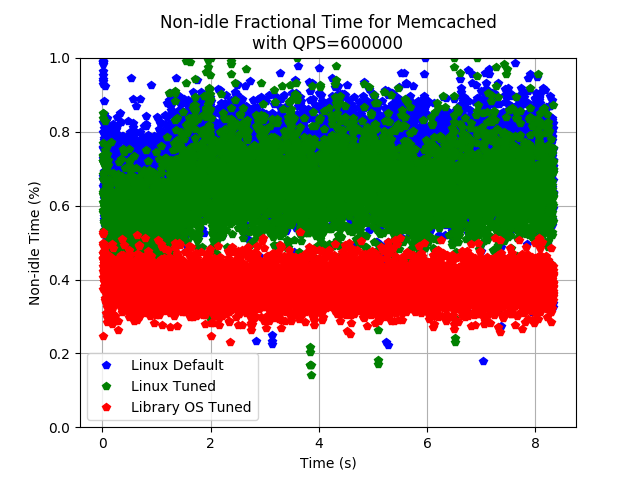
\includegraphics[width=\columnwidth]{asplos2021_figures/mcd_nonidle_QPS600000.png}
%% 	\caption{Per interrupt measure of non-idle time computed using fixed reference cycles.}
%% 	\label{fig:mcdnonidle600K}
%% \end{figure}

